% BLAKE3 extendable output [BLAKE3, §2.6]: the root node's compression is repeated with the
% ROOT flag and counters 0, 1, 2, ...; each full 16-word output gives 64 bytes.
% Original drawing for the Hash library.
\documentclass[tikz,border=6pt]{standalone}
\usepackage[T1]{fontenc}
\usepackage{lmodern}
% Shared style for the Hash diagrams.
% Palette: Okabe–Ito (colour-blind safe). Every diagram is drawn on an opaque white card so it
% stays legible on dark page themes.
\usetikzlibrary{arrows.meta,positioning,calc,fit,backgrounds}
\definecolor{hsblue}{HTML}{0072B2}
\definecolor{hsorange}{HTML}{E69F00}
\definecolor{hsgreen}{HTML}{009E73}
\definecolor{hsvermilion}{HTML}{D55E00}
\definecolor{hspurple}{HTML}{CC79A7}
\definecolor{hsink}{HTML}{1F2933}
\tikzset{
  >={Stealth[length=2.2mm]},
  every node/.style={font=\sffamily\small, text=hsink},
  wire/.style={draw=hsink, line width=0.6pt, ->},
  reg/.style={draw=hsink, line width=0.6pt, fill=hsblue!12, minimum width=9mm, minimum height=7mm},
  fn/.style={draw=hsink, line width=0.6pt, fill=hsorange!25, rounded corners=2pt, minimum width=10mm, minimum height=6mm},
  input/.style={draw=hsink, line width=0.6pt, fill=hsgreen!20, minimum width=9mm, minimum height=6mm},
  add/.style={circle, draw=hsink, line width=0.6pt, fill=white, inner sep=0pt, minimum size=5mm, font=\sffamily\bfseries},
  card/.style={fill=white, rounded corners=4pt},
}

\begin{document}
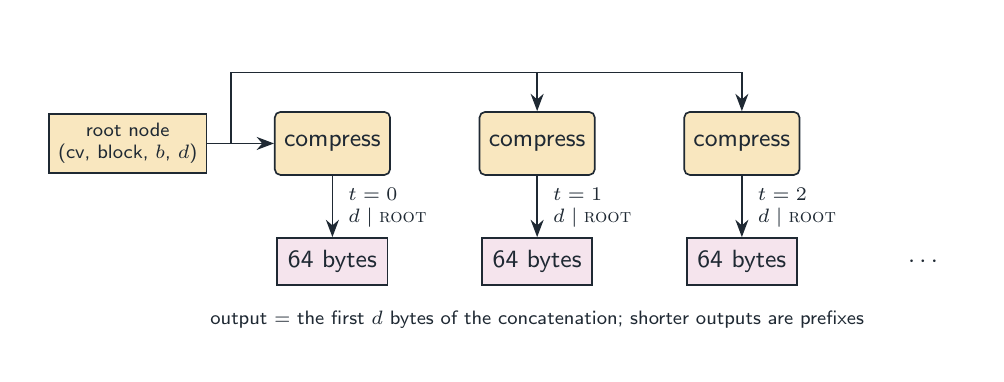
\begin{tikzpicture}
  \def\dx{2.6}
  \node[reg, fill=hsorange!25, align=center, font=\sffamily\scriptsize] (root) at (0,0)
    {root node\\(cv, block, $b$, $d$)};
  \foreach \i in {0,1,2} {
    \node[fn, minimum width=13mm, minimum height=8mm] (F\i) at (\i*\dx+2.6, 0) {compress};
    \node[font=\sffamily\scriptsize, anchor=west, align=left] at ($(F\i.south)+(0.08,-0.4)$) {$t = \i$\\$d \mid \textsc{root}$};
    \node[input, fill=hspurple!20, minimum width=14mm] (O\i) at (\i*\dx+2.6, -1.5) {64 bytes};
    \draw[wire] (F\i) -- (O\i);
  }
  \draw[wire] (root.east) -- (F0.west);
  \draw[wire] (root.east) -- ++(0.3,0) |- ++(0,0.9) -| (F1.north);
  \draw[wire] (root.east) -- ++(0.3,0) |- ++(0,0.9) -| (F2.north);
  \node[font=\sffamily\small] at (3*\dx+2.3, -1.5) {$\cdots$};
  \node[font=\sffamily\scriptsize, anchor=north] at (1*\dx+2.6, -2.0)
    {output = the first $d$ bytes of the concatenation; shorter outputs are prefixes};
  \begin{scope}[on background layer]
    \coordinate (e1) at (-1.2,-2.6);
    \coordinate (e2) at (3*\dx+2.9,1.4);
    \node[card, fit=(e1)(e2), inner sep=2pt] {};
  \end{scope}
\end{tikzpicture}
\end{document}
